\documentclass[a4paper, 11pt]{article}

\newcommand{\languages}{english, french}

%%%%% Tools

\usepackage{comment}
\usepackage{lipsum}
\usepackage{xstring}

%%%%% Document

\usepackage[pdfusetitle]{hyperref}

\usepackage{geometry}
\geometry{paper=a4paper,top=2.5cm,bottom=2.5cm,right=2.5cm,left=2.5cm}

\usepackage{fancyhdr}
%\pagestyle{fancy}
%\fancyhead[L]{}
%\fancyhead[R]{\leftmark}
%\fancyfoot[C]{\thepage}
%\renewcommand{\headrulewidth}{0pt}

%%%%% Text

\usepackage[utf8]{inputenc}
\usepackage[T1]{fontenc}
\edef\restoreparindent{\parindent=\the\parindent\relax}
\usepackage[parfill]{parskip}
%\restoreparindent
\usepackage{csquotes}

\newlength{\mytextsize}
\makeatletter
\setlength{\mytextsize}{\f@size pt}
\makeatother

%%%%% Languages

\ifx\languages\undefined
	\usepackage[english]{babel}
\else
	\usepackage[\languages]{babel}
\fi

% english

\addto\captionsenglish{\def\figurename{Figure}}
\addto\captionsenglish{\def\tablename{Table}}

\def\st{\text{s.t.}}

% french

\frenchbsetup{StandardLists=true}

\addto\captionsfrench{\def\figurename{Figure}}
\addto\captionsfrench{\def\tablename{Table}}
\addto\captionsfrench{\def\proofname{Preuve}}

\def\tq{\text{t.q.}}
\def\cad{c.-à-d.}
\def\Cad{C.-à-d.}

%%%%% Styles

\usepackage[skip=\mytextsize]{caption}
\usepackage{float}
\usepackage{mdframed}
\usepackage{enumitem}
\usepackage{eurosym}
\usepackage{color}

\newcommand\caaption[1]{\caption{#1}\vspace{-1\mytextsize}}

%%%%% Mathematics

\usepackage{amsmath}
\usepackage{amssymb}
\usepackage{amsfonts}
\usepackage{bm}
\usepackage{esint}
\usepackage[makeroom]{cancel}

\newcommand{\fact}[1]{#1!}
\newcommand{\e}[1]{\mathbf{e}_{#1}}
\newcommand{\deriv}{\mathrm{d}}
\DeclareMathOperator{\tr}{tr}


%%%%% SI units

\usepackage[squaren,Gray,cdot]{SIunits}
\usepackage{sistyle}

\IfStrEq{\languagename}{french}{
	\SIdecimalsign{,}
}

%%%%% Chemistry

\usepackage[version=4]{mhchem}

%%%%% Table & Figure

\usepackage{subcaption}

\usepackage{array}
\usepackage{tabularx}
\usepackage{multirow}
\usepackage{multicol}
\newcolumntype{M}[1]{>{\centering\arraybackslash}m{#1}}
%\setlength\extrarowheight{0em}
\renewcommand{\arraystretch}{1.3}

\usepackage{pgfplots}
\usepackage{tikz}
\usetikzlibrary{shapes.geometric, positioning}
\usepackage{graphics}
\usepackage{graphicx}
\pgfplotsset{axis on top, compat = 1.3}

%%%%%% Theorems and Definitions

\usepackage{amsthm}
\usepackage{thmtools}

\def\lgthm{Theorem}
\def\lglem{Lemma}
\def\lgprop{Proposition}
\def\lgdefn{Definition}
\def\lghyp{Hypothesis}
\def\lgquest{Question}
\def\lgansw{Answer}
\def\lgexpl{Example}
\def\lgrmk{Remark}
\def\lgnote{Note}
\def\lgtip{Tip}

\IfStrEq{\languagename}{french}{
	\def\lgthm{Théorème}
	\def\lglem{Lemme}
	\def\lgprop{Proposition}
	\def\lgdefn{Définition}
	\def\lghyp{Hypothèse}
	\def\lgquest{Question}
	\def\lgansw{Réponse}
	\def\lgexpl{Exemple}
	\def\lgrmk{Remarque}
	\def\lgnote{Note}
	\def\lgtip{Conseil}
}

\theoremstyle{plain}
\newtheorem{thm}{\lgthm}[section]
\newtheorem{lem}{\lglem}[section]
\newtheorem{prop}{\lgprop}[section]

\theoremstyle{definition}
\newtheorem{defn}{\lgdefn}[section]
\newtheorem{hyp}{\lghyp}[section]
\newtheorem{quest}{\lgquest}[]

\declaretheorem[
name=\lgansw,
qed={\lower-0.3ex\hbox{$\triangle$}},
within=quest
]{answ}

\declaretheorem[
name=\lgexpl,
qed={\lower-0.3ex\hbox{$\triangle$}},
within=section
]{expl}

\theoremstyle{remark}
\newtheorem*{rmk}{\lgrmk}
\newtheorem*{note}{\lgnote}
\newtheorem*{tip}{\lgtip}

\begingroup
\makeatletter
\@for\theoremstyle:=definition,remark,plain\do{%
	\expandafter\g@addto@macro\csname th@\theoremstyle\endcsname{%
		\addtolength\thm@preskip\parskip
	}%
}
\endgroup

%%%% Others

\renewcommand{\qedsymbol}{$\blacksquare$}

\newcommand{\mytableofcontents}{
	\newpage
	\pagenumbering{roman}
	\tableofcontents
	\newpage
	\pagenumbering{arabic}
}

%%%%%%%%%%%%%%%%%%%

%%%%%%%%%%%%%%%%%%%

\title{Introduction to artificial intelligence\\Pacman - Minimax agent}
\author{Maxime \textsc{Meurisse} (20161278)\and Valentin \textsc{Vermeylen} (20162864)}
\date{Academic year 2018-2019}

%%%%%%%%%%%%%%%%%%%

\begin{document}
    % ---------- Title page ---------- %
    \maketitle
	
	% ---------- Formalization of the problem ---------- %
	\section{Formalization of the problem}
	
	%\subsection{The basic problem}
	%The problem is in the form of a turn-taking game between Pacman and a ghost, both called \og agent\fg{}. Pacman's goal is to eat all food dots by avoiding being caught by the ghost. The play area is a labyrinth in which players and food dots are located.
	
	\subsection{Formalization as an adversarial search problem}
	This game can be formalized as an adversarial search problem composed of an initial state, a player function, a description of the possible actions for an agent state, a transition model, a terminal test and a utility function.\par
	
	Let us specify these components in the case of our problem:
	\begin{itemize}
	    \item initial state of the game: the starting position of all agents in the grid (defined by the layout, i.e. the game grid with food dots) and a boolean matrix of food dots;
	    \item the function player: a function that returns a numerical value associated with the agent that has to play (0 for Pacman, and 1 for the ghost);
	    \item possible actions for a given state: all agents can move in 4 directions: North, South, West and East or may not move. If a move leads Pacman into a wall, it is said to be an illegal move, otherwise it is a legal move;
	    \item transition model: thanks to one of the four previous actions, all agents update their position in the labyrinth (only one agent updates its position when it is its turn to play). Pacman possibly updates the boolean state of a food dot or dies because of a ghost;
	    \item terminal state: check if all food dots have been eaten, i.e. if all the food dots matrix is composed of false value (in this case, Pacman wins) or check if Pacman has been eaten by a ghost (in this case, Pacman loses);
	    \item utility function: this function assigns a numerical value to a state (the Pacman score associated to the state) that leads Pacman to a winning or a losing state. In case of a cycle, the value is + or - \(\infty\) depending of the current player.
	\end{itemize}
	
	
	% ---------- Performance of algorithms ---------- %
	\newpage
	
	\section{Performance of algorithms}
	The algorithms were run\footnote{The algorithms were run on a machine equipped with an 3.1 GHz Intel Core i7 processor with 16 GB of RAM.} on the \texttt{small\_adv} layout against the 3 ghost agents to study and compare their performance. All reported data is an average of 10 similar data.
	
	\begin{figure}[!ht]
	    \centering
	    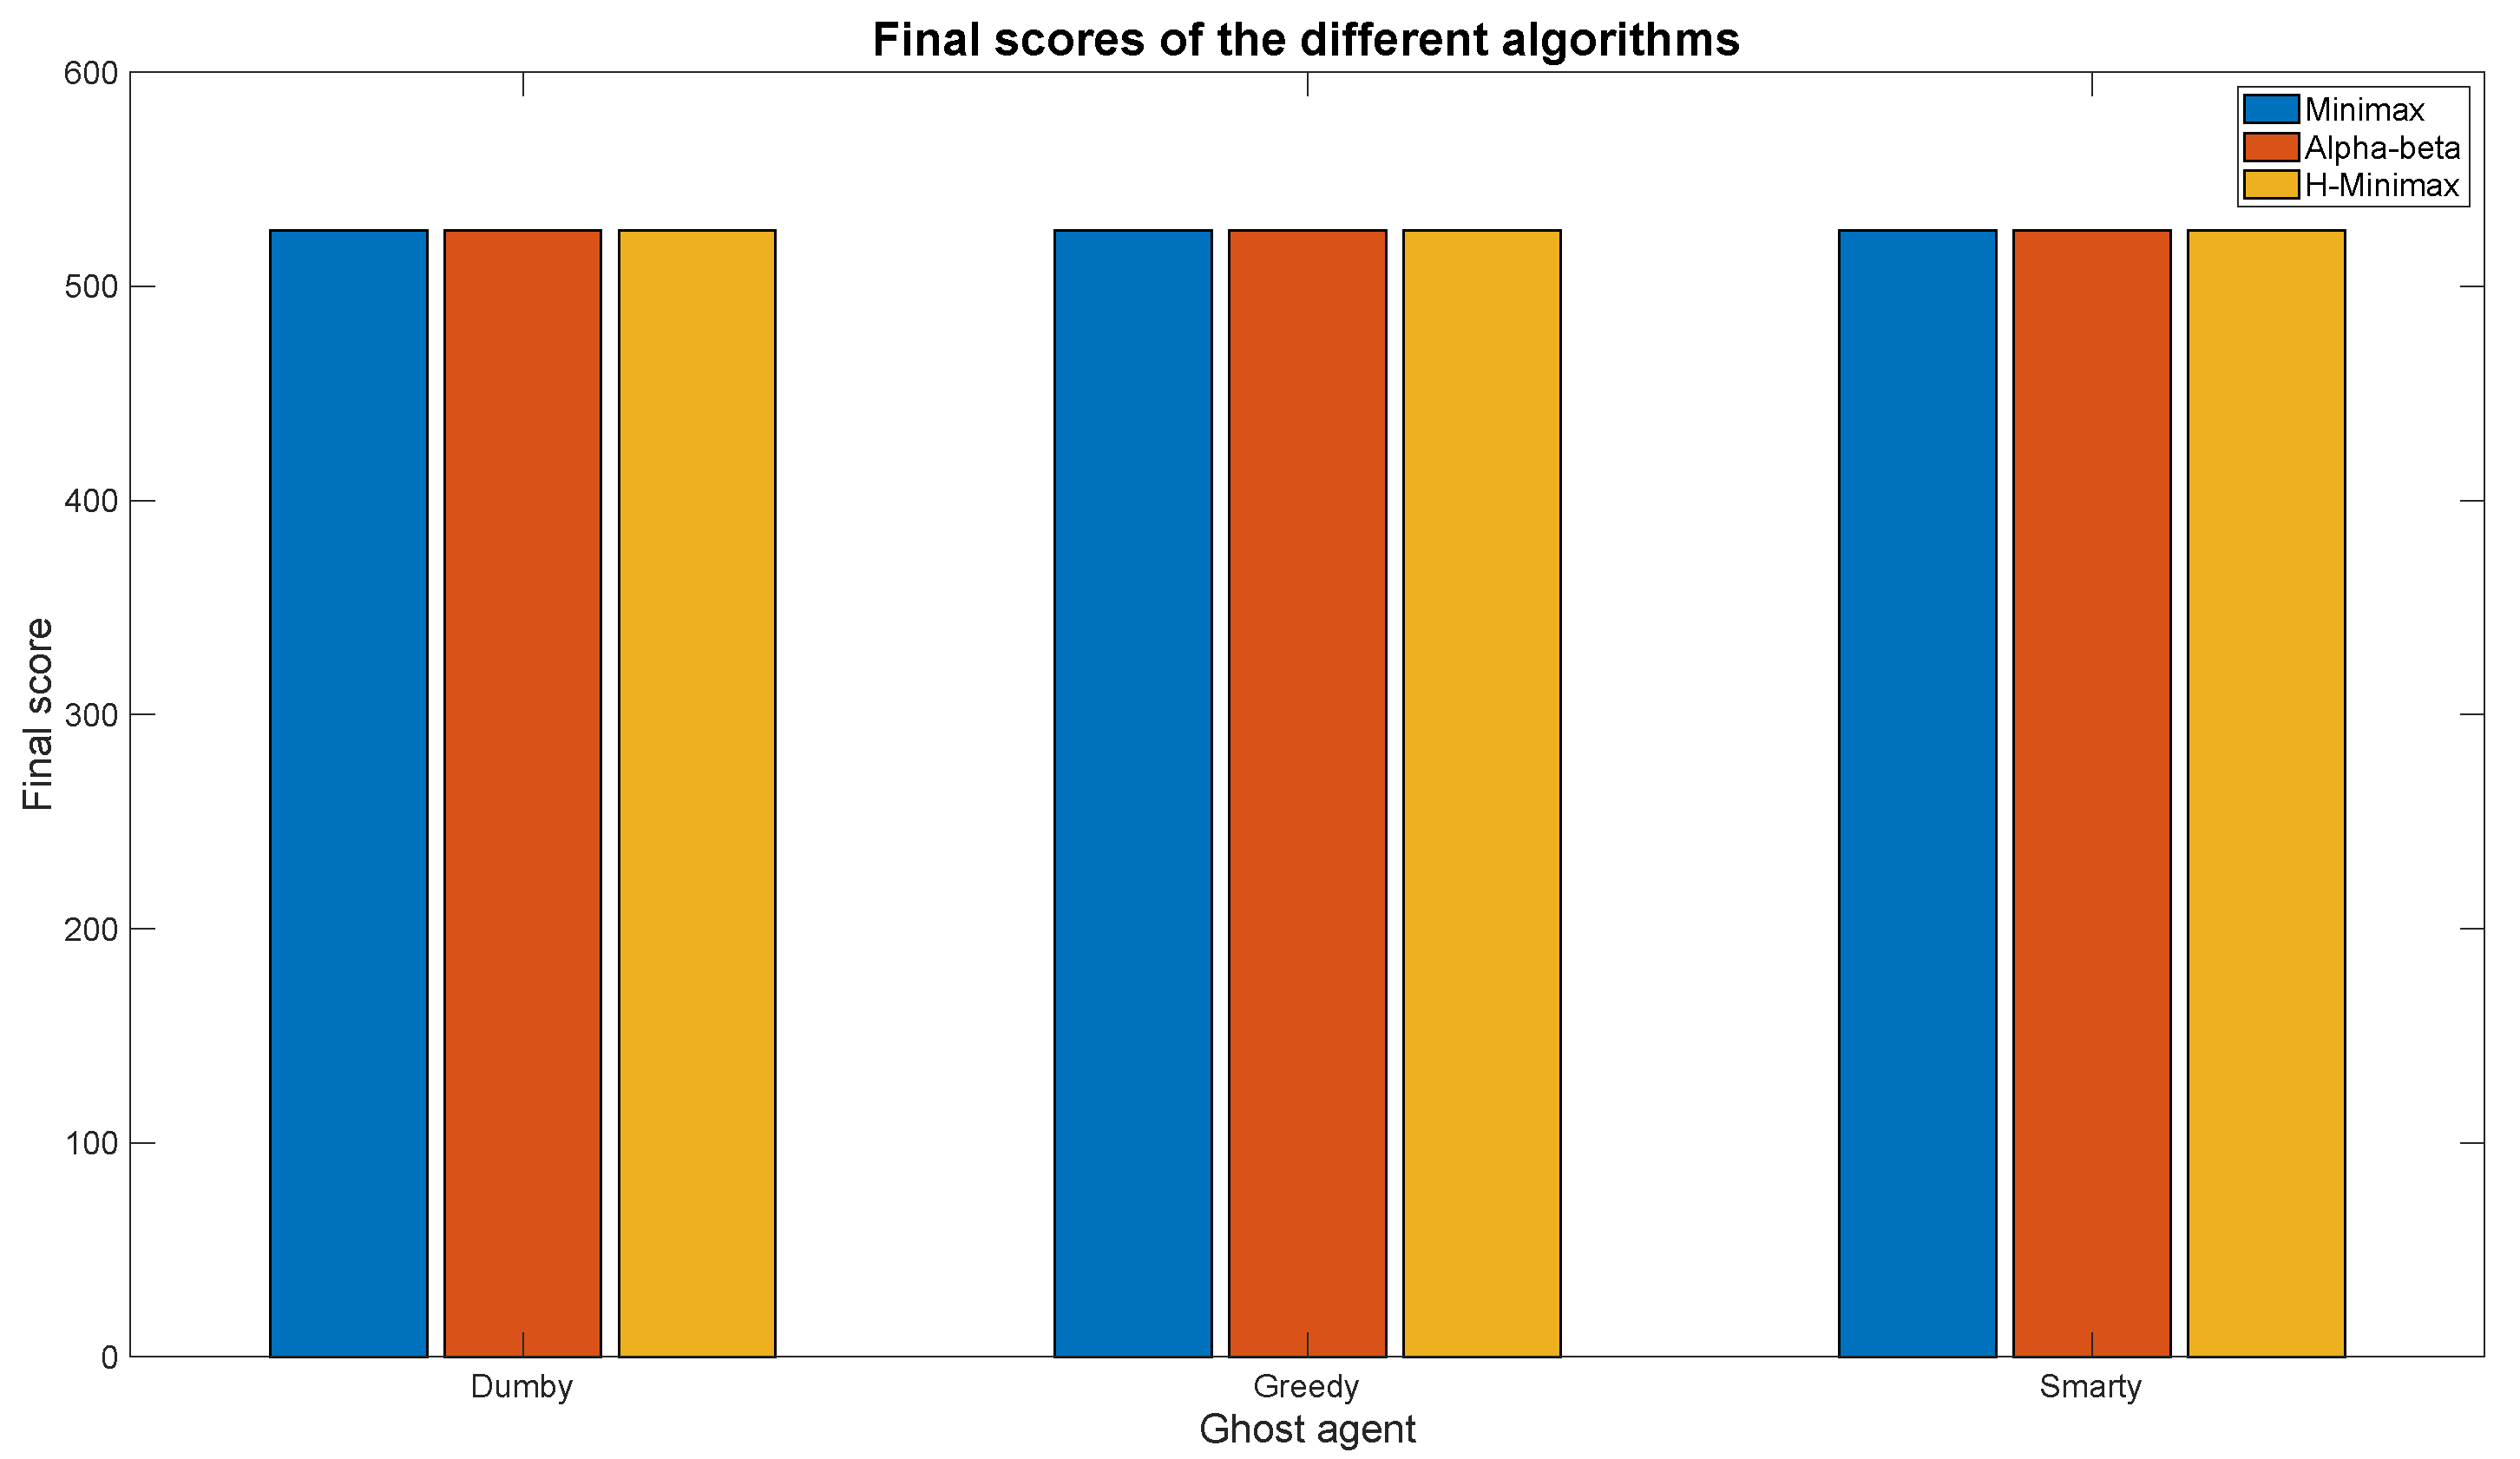
\includegraphics[width=0.75\textwidth]{resources/pdf/scores.pdf}
    	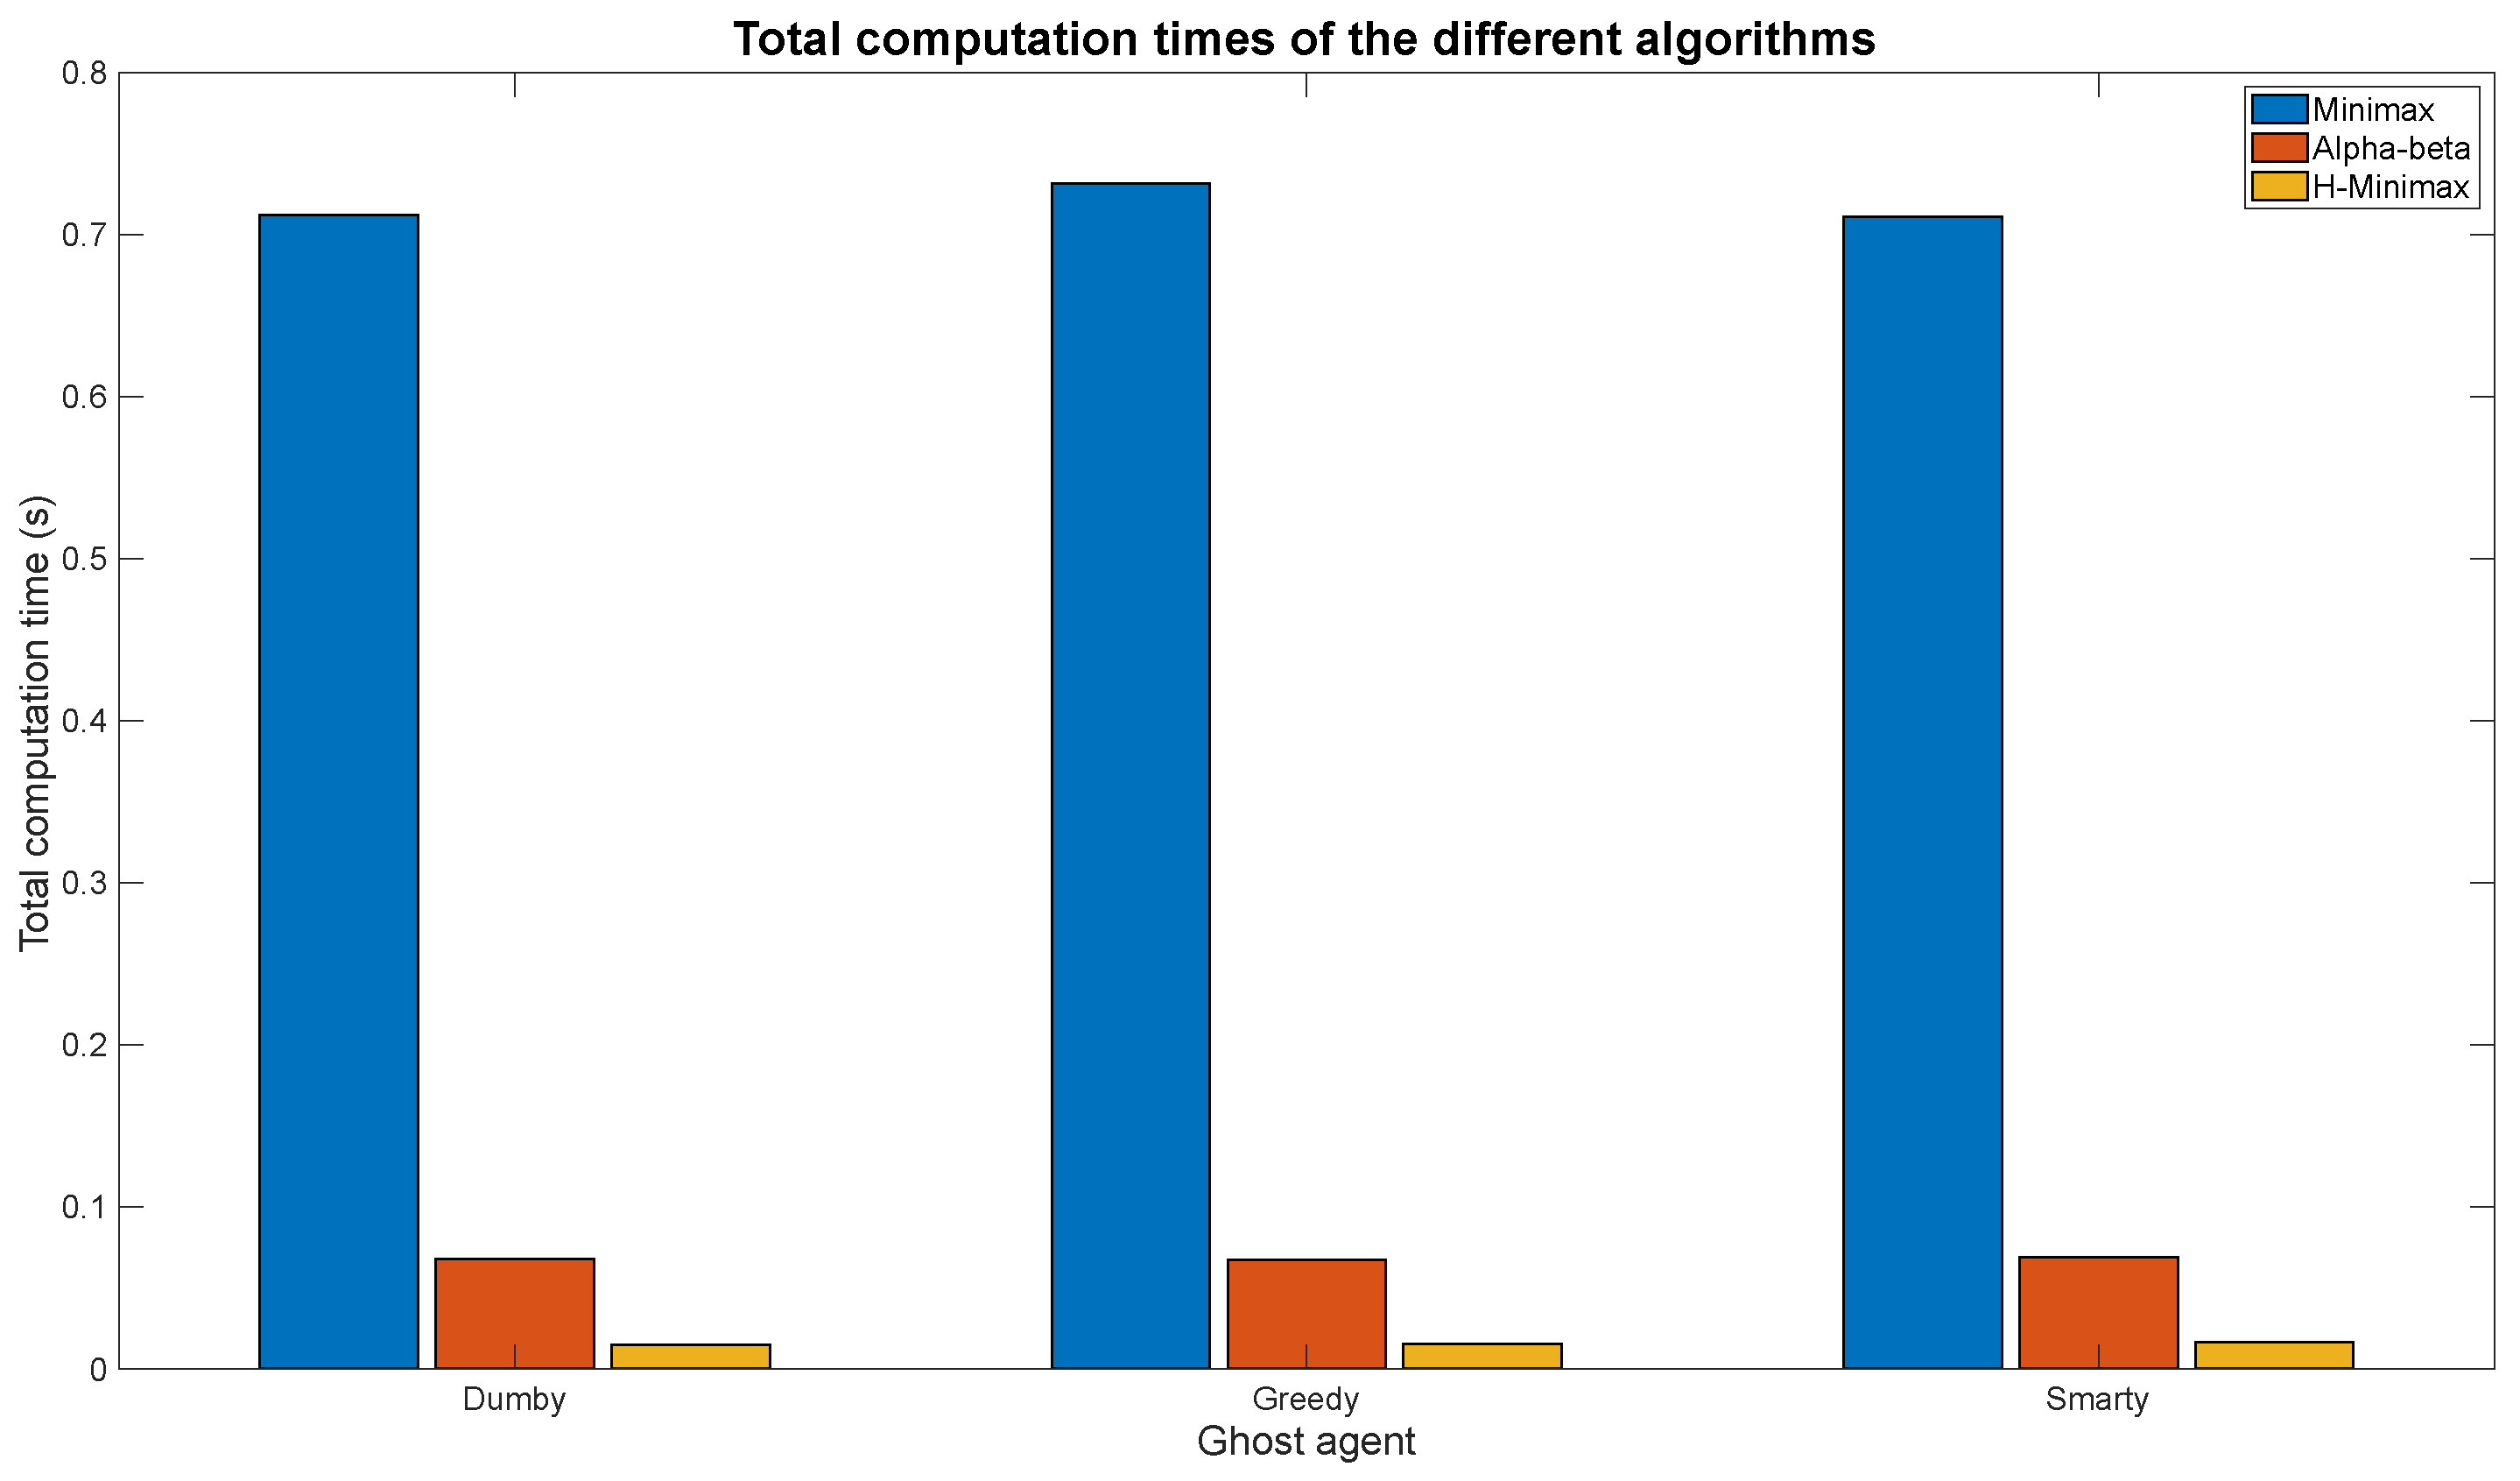
\includegraphics[width=0.75\textwidth]{resources/pdf/times.pdf}
        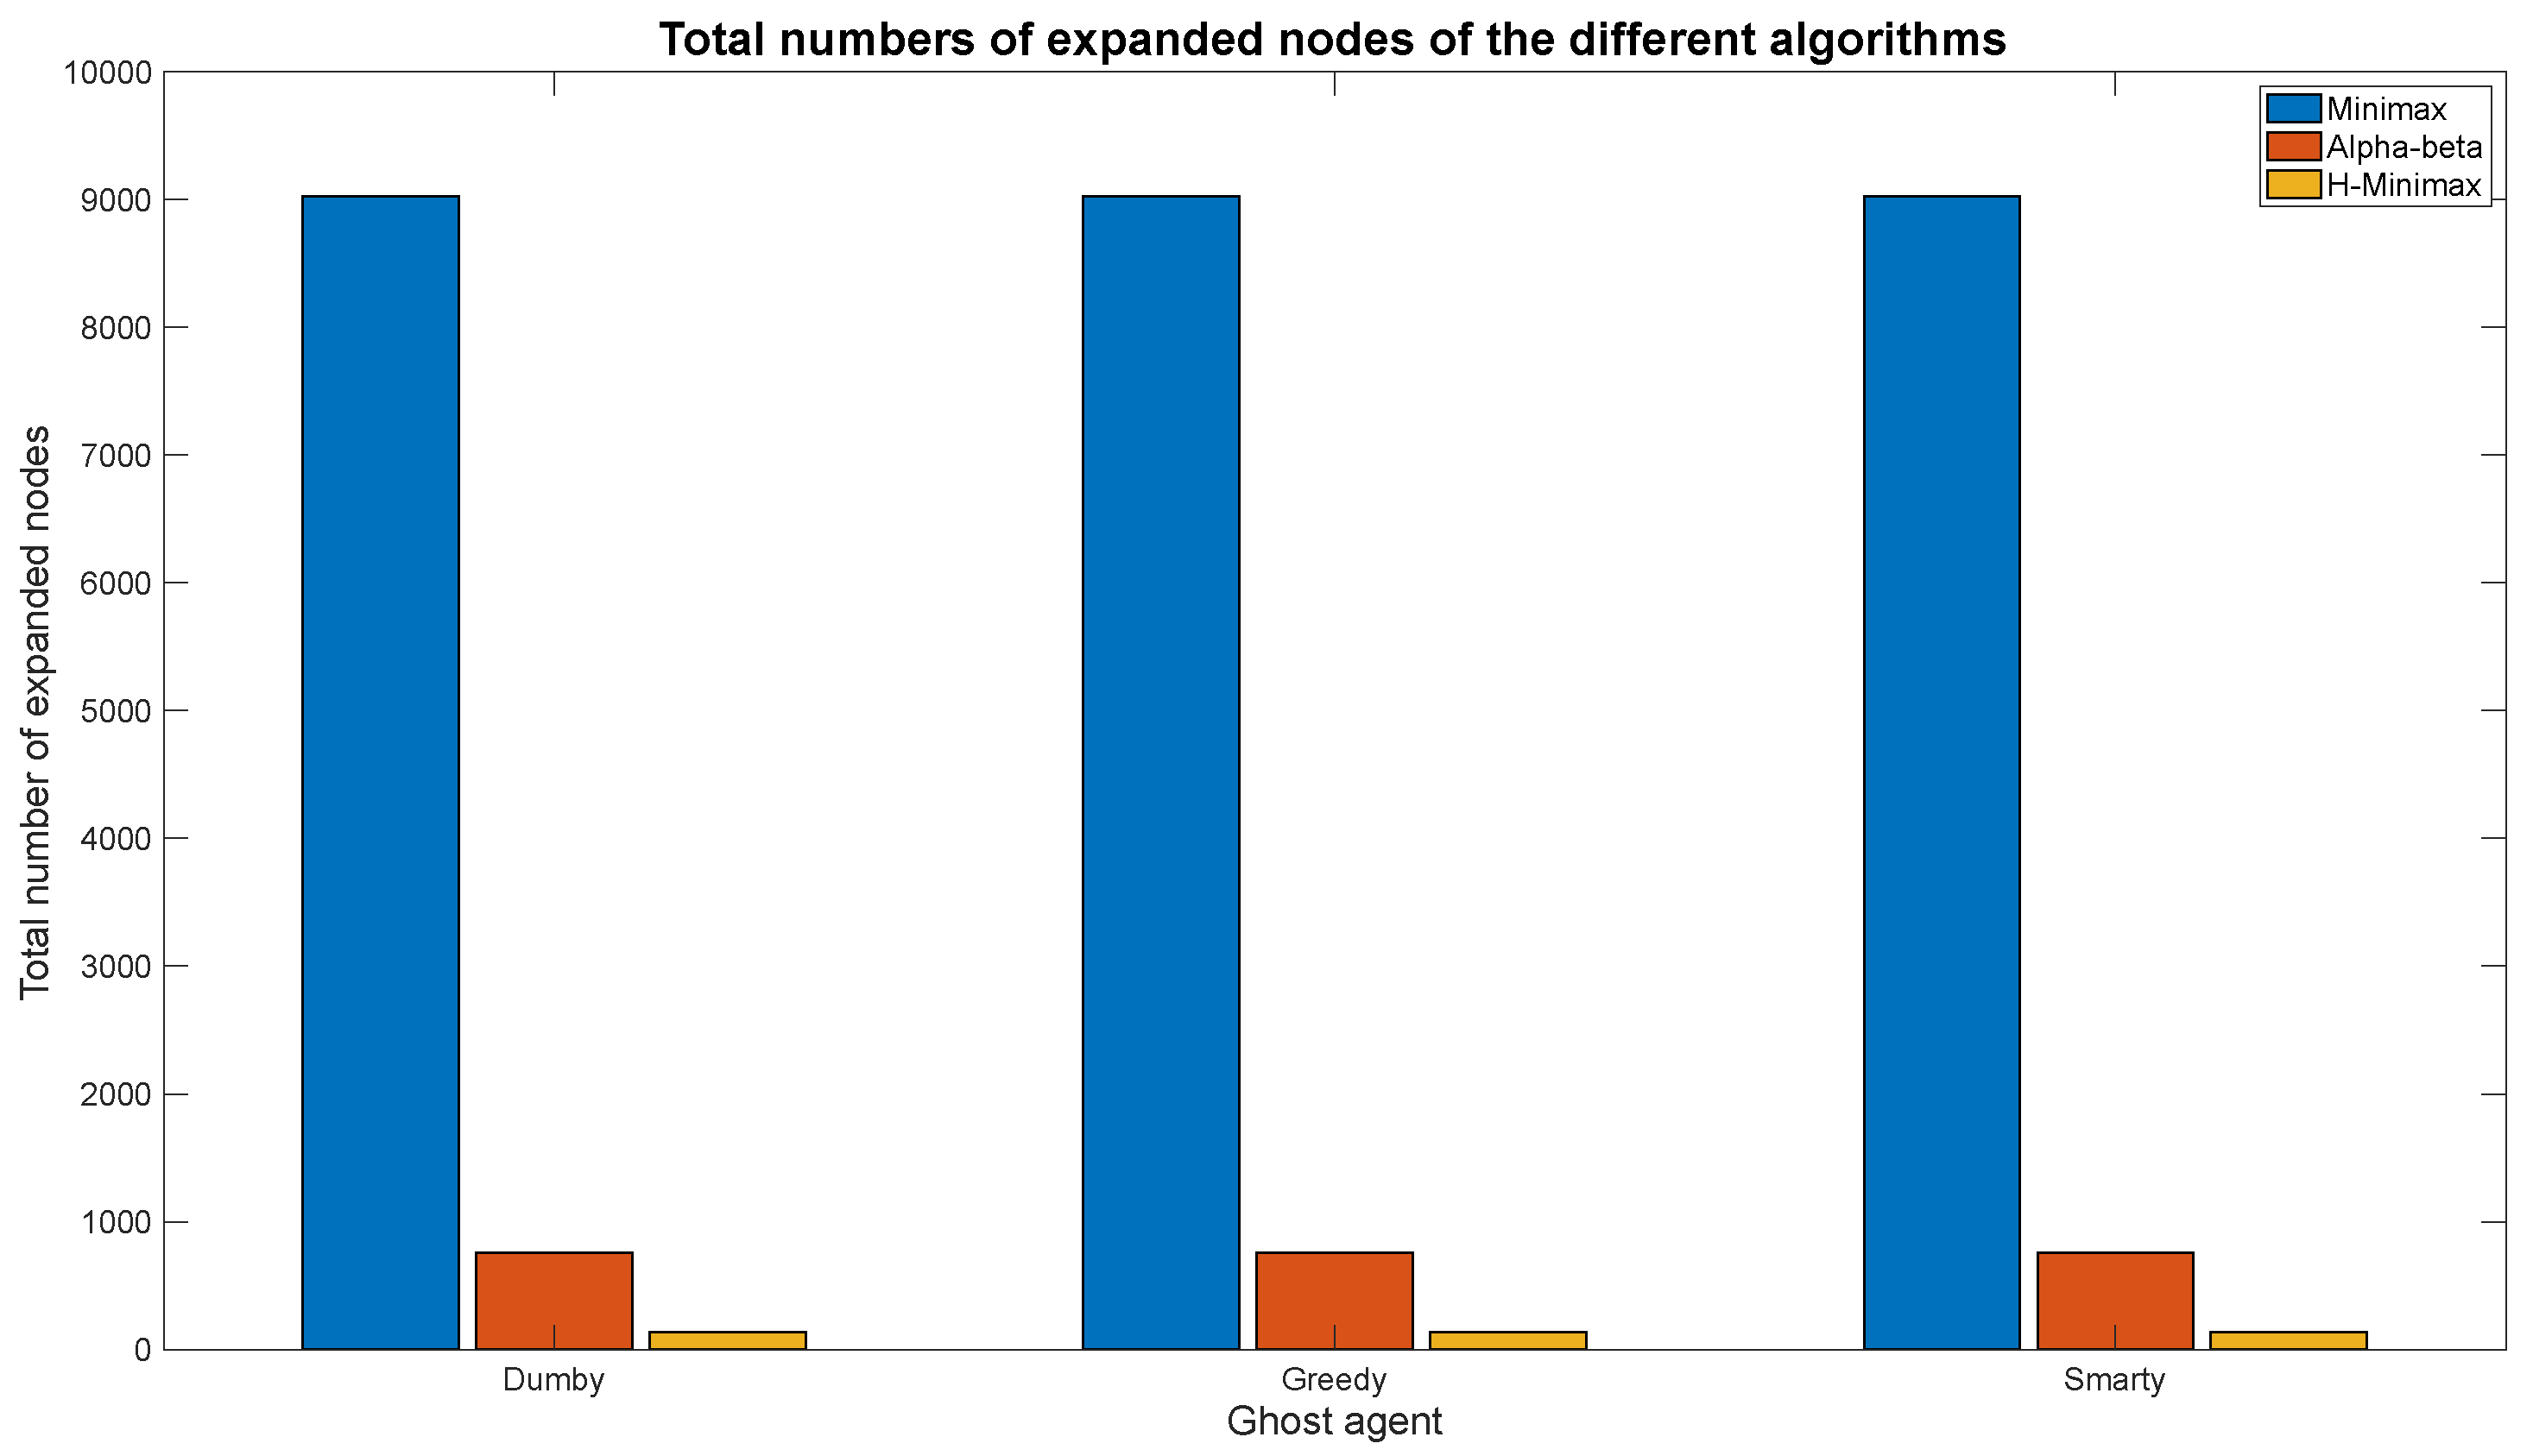
\includegraphics[width=0.75\textwidth]{resources/pdf/nodes.pdf}
        \label{fig:plots}
    \end{figure}
	
	
	% ---------- Discussion ---------- %
	\section{Discussion}
	
	\subsection{Minimax}
	
	As can be seen on the different graphs reported on section 2, \texttt{minimax} is the algorithm that expands the most nodes and has the most computation time, while all three find the same solution (the optimal one in this case). That can easily be understood as minimax is a recursive algorithm that needs to expand every child node until reaching a winning/losing/cycling node. We defined a cycle as a state (position of all agents and food dots matrix) being identical to one of its ancestor. In that case, we return + or - $\infty$ depending if the node is a child of, respectively, a minimizing or maximizing agent. 
	
	The solution is optimal because minimax is designed to maximize the score if competing against an optimal opponent. The opponent being suboptimal, we could have an even greater score than the one that could be obtained competing against an optimal one, but the layout is too small to see that. 
	
	However, even though minimax is optimal or better in this game, it cannot be applied to larger layouts without needing lots of computation time and memory space (because it is recursive). As it could not be launched against the provided layouts, we created 4 new ones to test our agent and it always chose to maximize its score by finding the optimal solution or dying when it understood that the opponent could send it into a cycle, decreasing indefinitely its score.
	
	\subsection{Alpha-beta}
	
	\texttt{Alphabeta} is simply \texttt{minimax} that does not expand useless nodes. For that reason, it expands way less nodes (and the computation time is reduced), and the ratio (expanded / all nodes) decreases as the layouts grow larger. The final score is always the same as that of minimax because the branches that have not been explored are simply the ones that would not have been reached in an actual game play, thus they do not influence the optimal score.
	
	Nevertheless, our implementation of alphabeta did not allow us to run it to completion on \texttt{medium\_adv}. It launched after increasing a bit the recursion limit of the system, but took way too long to calculate its first move (and had not finished when we killed it). For that reason, we launched it on the same personal layouts than minimax and made the same observation as before.
	
	\subsection{H-Minimax}
	
	We decided to implement our \texttt{hminimax} with alpha-beta pruning, reducing the nodes expanded and the computation time. That can easily be seen on the graphs. With a depth of 10 (8 was enough but 10 is safer if you are to run it on larger layouts), we reached an optimal solution on the small layout for all ghosts as their behaviour does not change anything on such a small maze. On the medium, it won against all ghosts. (Dumby : score : 539, nb of nodes expanded : 48664, time : 9.007s ;
Greedy : score : 539, nb of nodes expanded : 30183, time : 5.58s
Smarty : score : 539, nb of nodes expanded : 29503, time : 5.44s)\newline
As can be seen from the data, the plays against smarty and greedy were quite similar as they have a similar behaviour. However, playing against dumby resulted in longer calculation and more expanded nodes as it has strange movement that are far from the optimal ones (as opposed to smarty and greedy that are not as far from optimal), which pacman expects. But it got the same score against all agents.
	
	On the large one, it won against dumby but lost against the others (That is further developed below.) (Dumby: score : 544, nb of nodes expanded : 153514, time : 34.47s ; 
Greedy: score : -450, nb of nodes expanded : 79813, time : 18.77s ; 
Smarty: score : -450, nb of nodes expanded : 79813, time : 18.81s)\newline
The same conclusions as above can be drawn concerning the number of expanded nodes and calculation time. However, Pacman wins only against dumby. That is further explained in the example below, but smarty and greedy are almost optimal in that play, and the layout is not winnable against an optimal opponent, which is why pacman loses, but maximizes its score before doing so.
	
	Our \textbf{evaluation function} is the following : 
	
	\texttt{value = score - 1.5 * food\_min - (2 / (ghost\_min)) - 4 * food\_number}
	
	Where \texttt{score} is the score associated with the state, \texttt{food\_min} is the smallest distance between a food dot and pacman, \texttt{ghost\_min} is the smallest distance between pacman and the closest ghost and \texttt{food\_number} is the number of food dots that are left on the grid.
	
	The evaluation function pushes Pacman to get closer to food dots and get away from the ghost(s). Furthermore, it gives pacman a greater penality the more food there is on the grid, forcing it to go get it.
	
	The function is partially adapted from \texttt{https://gist.github.com/dcalacci/6953749}. We initially only took into account the distance to the ghost and the distance to the nearest food dot, but the problem was that it would get stuck against walls with a food dot on the other side. Being rewarded when eating a dot solved that problem.
	
	
	Concerning the \textbf{cutoff function}, we decided to cut the search if the state was in a winning or losing end, if the depth of the branch was greater than a limit, or if we were cycling. What we mean by circling is that if we ended up in the same state (position of all agents and food dot matrix) as an ancestor, we would cut the search, as the solution could not be optimal (or not optimal enough).
	
	The cycling condition is a way to speed the algorithm but does not impact the solution. It is the same cycle avoidance than the one used in minimax and alphabeta.
	
	We also tried to implement a test that checked if Pacman was directly next to a ghost after one of its movement but we did not keep it. However, it could be an improvement.
	
	Another test we added was a check to see whether Pacman was 1 block apart from the ghost when we cut the search (meaning he would die at the next ghost move). We wanted to make sure the algorithm was quiescent but realized that it changed nothing as our evaluation function takes care of moving Pacman away from the ghost. It simply resulted in more nodes expanded. However, if we are wrong about that, it could easily be implemented back.
	
	What is worth noting is that the depth used to cut the search has a great impact on our solution. A small depth (5 or less) will lead our agent to become more greedy, as he will prefer eating dots and coming closer to them (due to our evaluation function). A greater depth (10 or more) will lead our agent to make better decisions and have an overall better score.
	
	An example of that is the large layout. For a small depth, the agent eats the dot that is closer to it. However, if we think about it, it is a suicide move against an optimal opponent as he will move right under the square wall and Pacman will inevitably die after 2 moves at most. The ghost being suboptimal, Pacman could still win using that strategy but it is not really correct, and it dies in our implementation, as it should.\newline
	Using a greater depth, Pacman goes to the left and eats all the dots except the one mentioned before. He then dies against smarty or greedy but with a greater score than the one he could have obtained against an optimal opponent by taking the first dot. (Against an optimal opponent, we believe that the large layout is not winnable. Pacman would get caught in a corner before eating all the dots.)
	
	Also, as we cut the search sooner, we stumbled upon a strange problem : Pacman started cycling for no reason while next to a dot (large layout, against dumby). That came from the fact that all child nodes of the initial state had the same value, thus Pacman would choose the first or last one depending on the inequality (> or >= changed the behaviour). Increasing the depth would result in cycles appearing later. That was not acceptable and might come from the cut in the tree, which is why we evaluated each son node and returned the action associated with the better one if we had the case.
\end{document}
